\documentclass[aspectratio=169]{beamer}
\usetheme{Madrid}
\usepackage{physics}
\usepackage{bm}
% Remove the automatic "Figure" label in captions for the presentation
\usepackage{caption}
\captionsetup[figure]{labelformat=empty}
\usepackage{xcolor} % ensure color package available
\usepackage{pifont} % for checkmark and cross
\definecolor{ff00ff}{HTML}{FF00FF} % define color #ff00ff
% Set background to black and all text to white
\definecolor{highlight}{HTML}{ffdb58} % new highlight color #ffdb58
\usecolortheme{default}
% set alerted text color (no bold)
%\setbeamercolor{alerted text}{bg=highlight}
% remove any bold setting: do NOT use \setbeamerfont{alerted text}{series=\bfseries}
% inline highlight: black text on colored background (with small padding)
\newcommand{\hlbg}[1]{\begingroup\setlength{\fboxsep}{3pt}\colorbox{highlight}{\strut\textbf{\textcolor{black}{#1}}}\endgroup}
% convenience macro for inline highlighted text (no bold)
\newcommand{\hl}[1]{{\color{highlight}#1}}
\newcommand{\cmark}{{\color{green!60!black}\ding{51}}}
\newcommand{\xmark}{{\color{red}\ding{55}}}

\definecolor{mywhite}{RGB}{255,255,255}
%\setbeamercolor{background canvas}{bg=white}
%\setbeamercolor{normal text}{fg=black}
% Define the blue color for footline
\definecolor{footlineblue}{HTML}{003DA5}

\setbeamercolor{frametitle}{bg=white, fg=footlineblue}
%\setbeamercolor{title}{bg=black, fg=mywhite}
%\setbeamercolor{section in toc}{fg=black}
%\setbeamercolor{subsection in toc}{fg=black}
%\setbeamercolor{item}{fg=black}
%\setbeamercolor{block title}{bg=black, fg=mywhite}
%\setbeamercolor{block body}{bg=black, fg=mywhite}

% Remove navigation symbols
\setbeamertemplate{navigation symbols}{}

% Remove the automatic section/subsection TOC at the top of each slide
\setbeamertemplate{headline}{}


% Show current slide number and total number of slides in footline

\definecolor{lightblue}{HTML}{D6E4F0}
% Show current slide number and total number of slides in footline
\begin{document}

\title[DL4Sci: Quantum Trajectory]{Proposal for Final Project:\\ Predicting open system quantum dynamics by learning on quantum trajectories}
%\email{nikita.leppanen@weizmann.ac.il}
\author[Nikita Leppenen]{Nikita Leppenen}
\institute[]{Department of Chemical \& Biological Physics \\ Weizmann institute of Science, Rehovot}
\date[\today]{\today}

\begin{frame}
    \titlepage
\end{frame}

\begin{frame}
    \frametitle{Physics (short): Driven-dissipative cavity QED}
    \begin{figure}
        \centering
        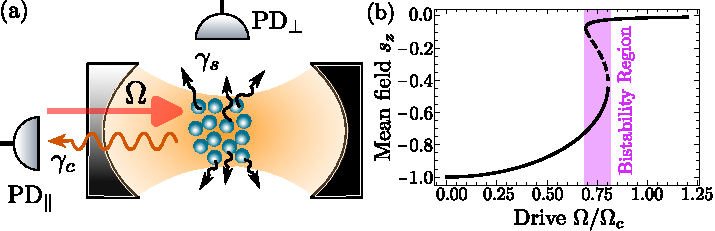
\includegraphics[width=0.8\textwidth]{img_1/fig_for_cavity.pdf}
        \caption{(a) System under study (b) Mean-field solution and bistability region}
    \end{figure}

    Main equation -- Master equation
    \begin{equation}
        \dot{\rho} = -i[{\cal H}, \rho] + \frac{\gamma_c}{2}{\cal D}[\hat{S}_-]\rho + \frac{\gamma_s}{2}\sum_n{\cal D}[\hat{\sigma}_n]\rho,\qquad {\cal H} = 2\Omega \hat{S}_x
    \end{equation}
\hfill{\scriptsize \underline{Leppenen}, Shahmoon, Phys. Rev. A 2026}
\end{frame}
\begin{frame}
    \frametitle{How to solve the master equation? Answer: MCWF method}

    Generally: Solve for density matrix: $4^N \times 4^N$ elements, $N$ is the number of qubits.\\
    Instead:
    Probabilistic unraveling of the master equation into quantum trajectories
    \begin{equation}
        \ket{\psi(t+dt)} = 
        \begin{cases}
            \frac{\hat{S}_-\ket{\psi(t)}}{\sqrt{p_-}} & \text{with probability } p_- = \gamma_c dt \langle \psi(t)|\hat{S}_+\hat{S}_-|\psi(t)\rangle \\
            \frac{\hat{\sigma}_n\ket{\psi(t)}}{\sqrt{p_n}} & \text{with probability } p_n = \gamma_s dt \langle \psi(t)|\hat{\sigma}_n^\dagger\hat{\sigma}_n|\psi(t)\rangle \\
            \frac{e^{-i{\cal H}_{NH}dt}\ket{\psi(t)}}{\sqrt{p_0}} & \text{with probability } p_0 = 1 - p_- - \sum_n p_n
        \end{cases}
    \end{equation}
    \cmark\ Saves memory: $2^N \times 2^N$ elements
    
    \xmark\ Loses Time: Need to average over many trajectories to get the density matrix.

    \vspace{1 cm}
    In our work we found that a bistability is seen in a single trajectory, but the bistability is lost in the density matrix average.
    \hfill{\scriptsize \underline{Leppenen}, Shahmoon, Phys. Rev. A 2026}
\end{frame}

\begin{frame}
    \frametitle{How typical trajectory looks like (in bistability case)}
    \begin{figure}
        \centering
        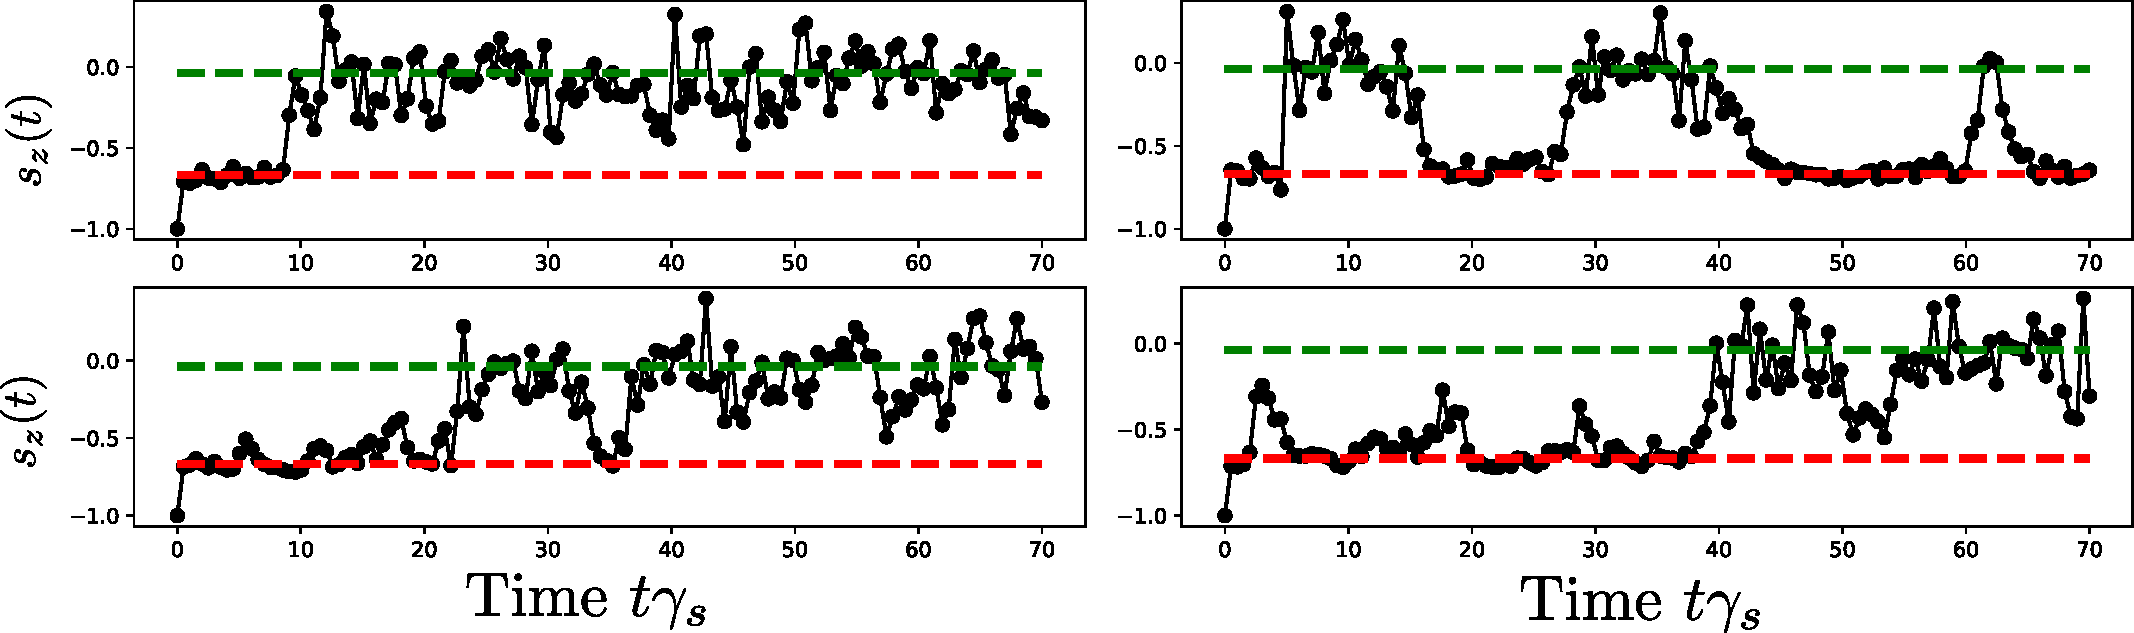
\includegraphics[width=\textwidth]{img_1/four_traj.pdf}
        \caption{4 examples of quantum trajectories $N = 18$ (best I can get), $\Omega = 0.73\Omega_c$ (bistability region), $\gamma_c = 10\gamma_s$. Red and Green lines are the mean-field solutions. Generated with QuTiP (python library for quantum simulations).}
    \end{figure}

    Note: average of $N_{tr} \approx 100$ trajectories gives the density matrix solution, which is a smooth curve (no bistability).
    \hfill{\scriptsize \underline{Leppenen}, Shahmoon, Phys. Rev. A 2026}
\end{frame}

\begin{frame}
    \frametitle{Problem statement}
      \begin{figure}
        \centering
        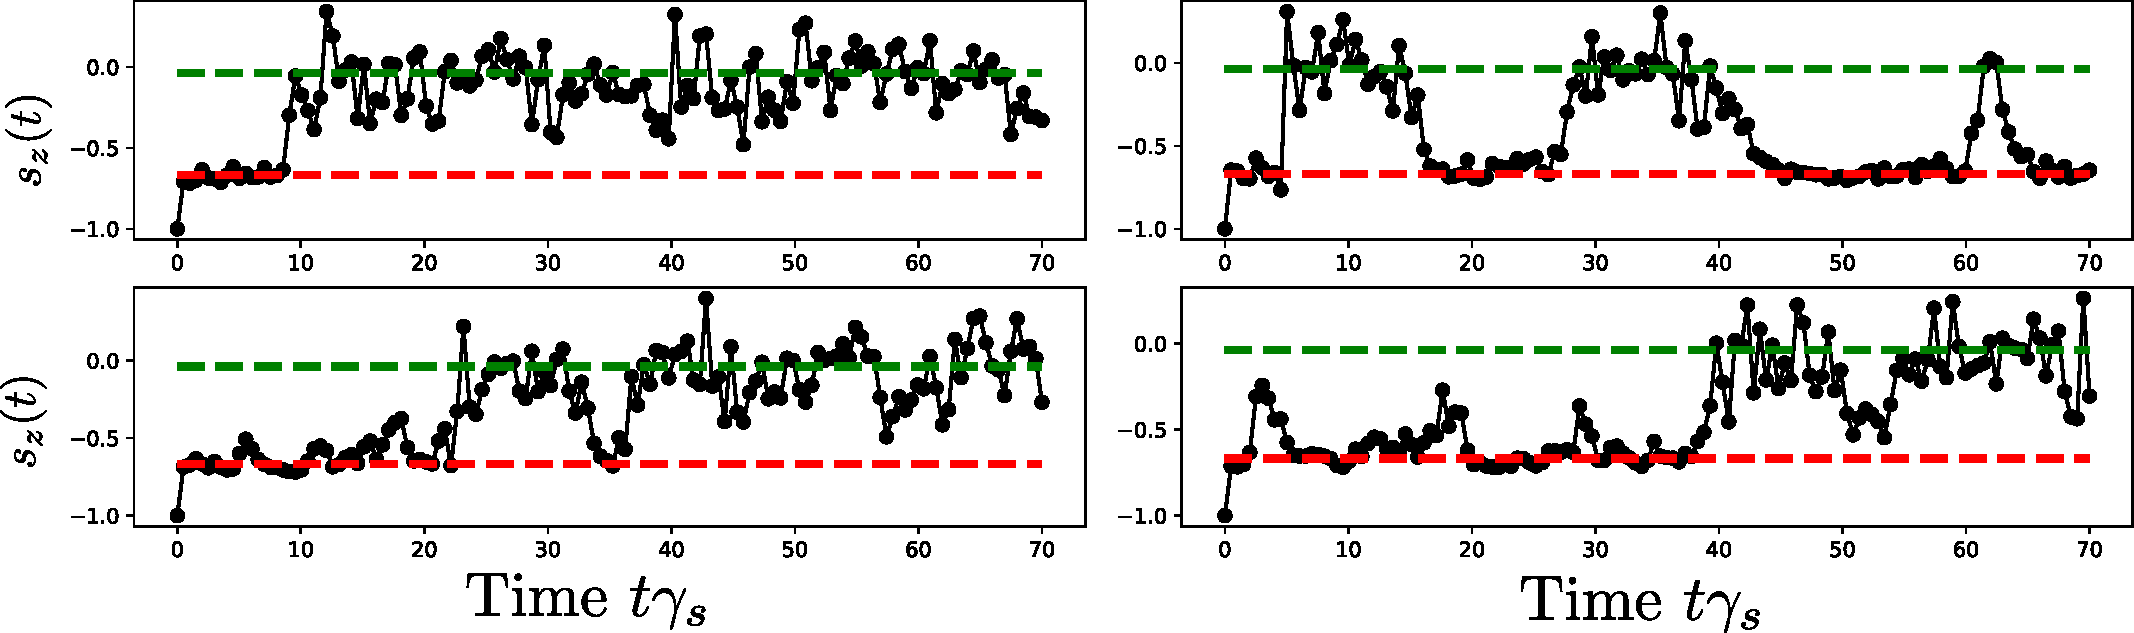
\includegraphics[width=\textwidth]{img_1/four_traj.pdf}
        \caption{4 examples of quantum trajectories $N = 18$ (best I can get), $\Omega = 0.73\Omega_c$ (bistability region), $\gamma_c = 10\gamma_s$.}
    \end{figure}  

    \vspace{-0.5cm}
    \begin{block}{Goal of the project}
        Create a model to generate trajectories similar to quantum trajectories generated by Monte Carlo wave-function simulations in QuTiP
    \end{block}
\end{frame}

\begin{frame}
    \frametitle{Why this matters?}
    \begin{figure}
        \centering
        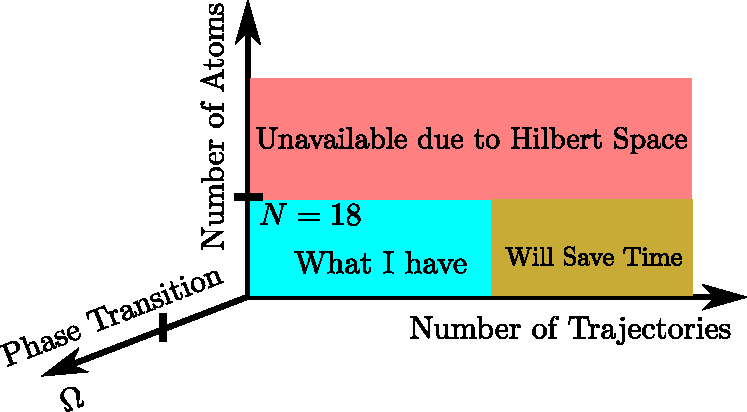
\includegraphics[width=0.8\textwidth]{img_1/logic1.pdf}
    \end{figure}
\end{frame}

\end{document}